\section{Aplicações da Integral}


\subsection*{Área entre curvas}


\begin{frame}{Área entre curvas}
Queremos determinar a área delimitada pelo gráfico de duas funções.



\begin{center}
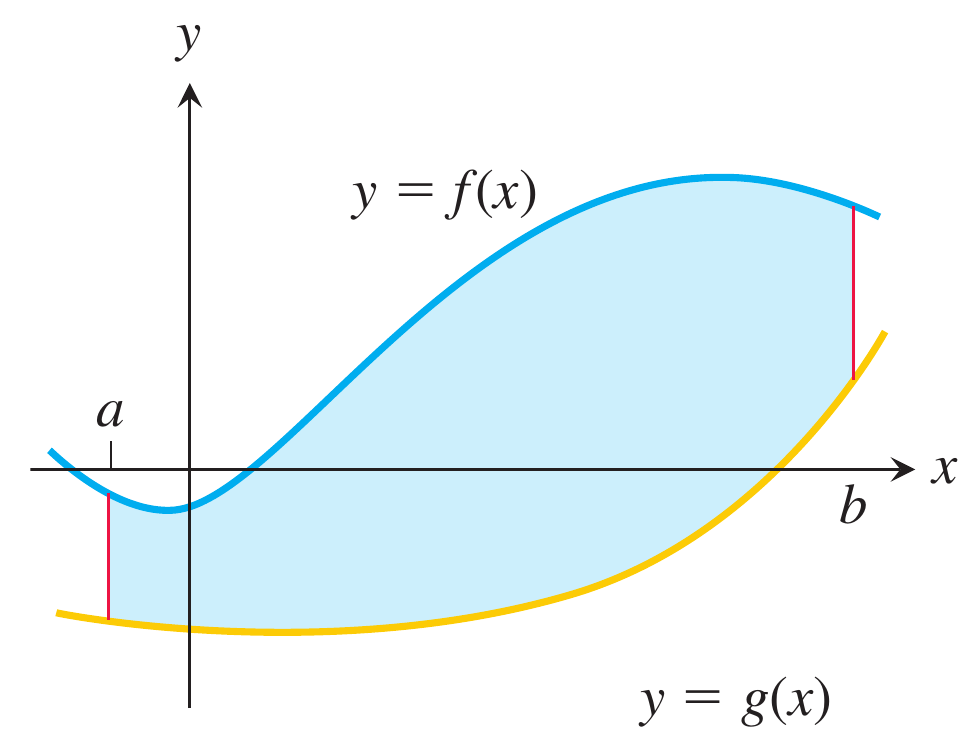
\includegraphics[scale=1]{area-curvas-th-1.png}
\end{center}
\end{frame}

\begin{frame}
No caso em que $f(x)\geq g(x)$ em $[a,b]$.

\begin{center}
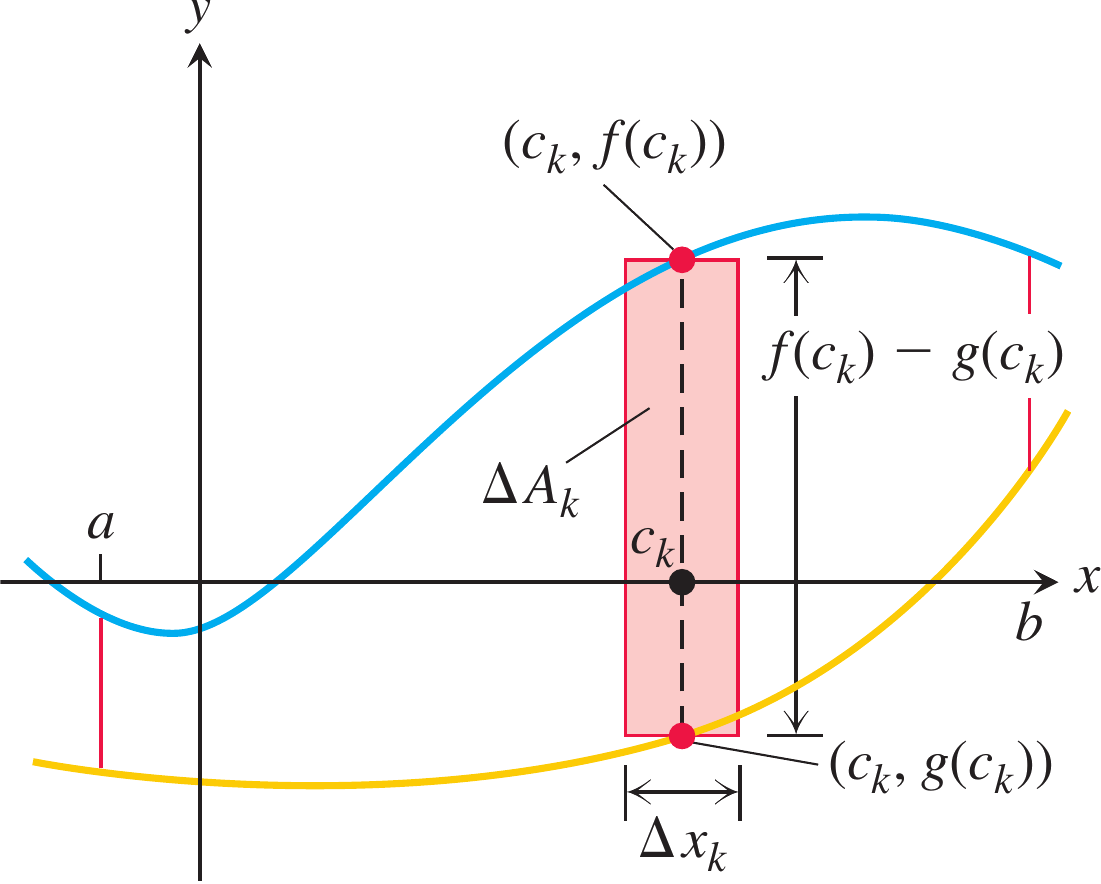
\includegraphics[scale=0.6]{area-curvas-th-3.png} \ \ \ 
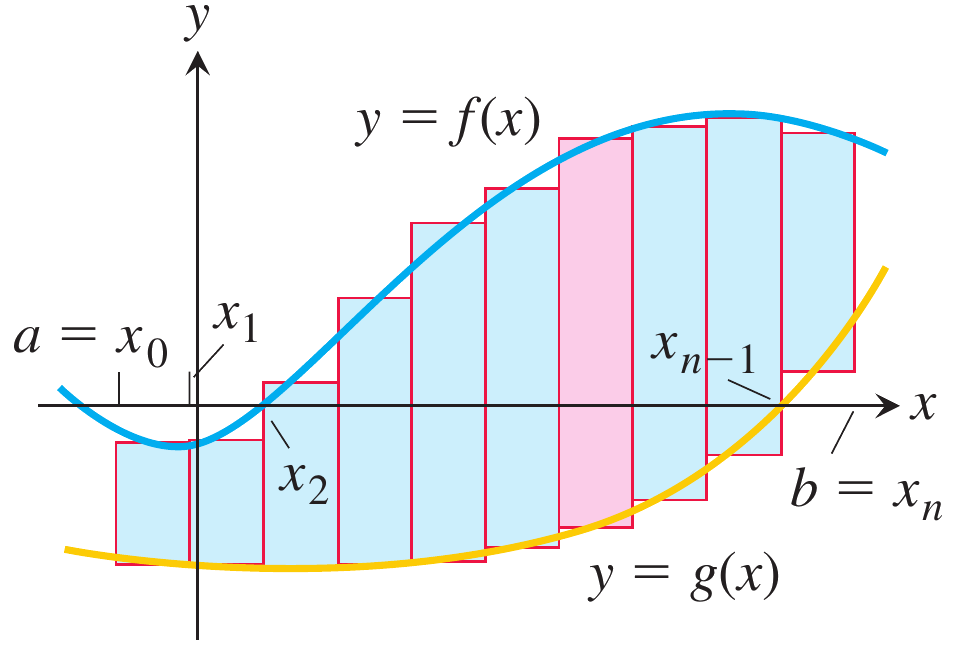
\includegraphics[scale=0.7]{area-curvas-th-2.png}
\end{center}

\[\text{Área}(S)=\lim_{\|P\|\to 0}\sum_{k=1}^{n}(f(c_k)-g(c_k))\Delta x_k=\int_a^b f(x)-g(x)dx\]
\end{frame}

%\begin{frame}
%\frametitle{Áreas entre curvas}
%%
%
%\uncover<1->{Vimos que se uma função não é negativa, então as somas de Riemann aproximam-se da área compreendida entre o gráfico da função e o eixo $OX$. Isso motiva a seguinte definição
%\begin{defin}
%Seja $f:[a,b]\to \R$ uma função integrável. A \dt{área} limitada pela curva $y=f(x)$ e o eixo $OX$ é dada por:
%$$\int_a^b|f(x)|dx$$
%\end{defin}}
%
%\begin{exe} 
% Calcule a área  limitada pela curva $y=x^2-x$ e o eixo $OX$ no intervalo $[0,2]$.
%\end{exe}
%
%%\uncover<1->{\begin{exe} 
%% Esboce o gráfico e calcule a área  limitada pela curva $y=x^3-x^2-2x$ e o eixo $OX$.
%%\end{exe}}
%
%
%\end{frame}
%
%
%\begin{frame}
%\begin{exer}
%Calcule a área limitada pela curva $y=\cos(x)$ e o eixo $OX$ no intervalo $[]$
%\end{exer}
%\end{frame}

\begin{frame}
\frametitle{Área entre curvas}



\begin{defin}
Sejam $f:[a,b]\to \R$ e $g:[a,b]\to \R$  funções integráveis. A \dt{área} limitada pelas curvas $y=f(x)$ e $y=g(x)$ e pelas retas $x=a$ e $x=b$ é dada por:
$$\int_a^b|f(x)-g(x)|dx$$
\end{defin}

\begin{center}
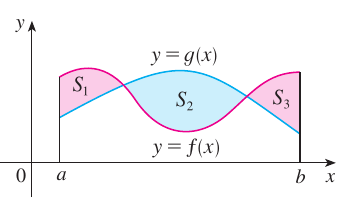
\includegraphics[scale=.7]{area-curvas.png}
\end{center}


\end{frame}

\begin{frame}

\begin{exe} 

 Determine a área limitada pelas curvas $y=2-x^2$ e $y=-x$.

%\item Determine a área entre a curva $y=x^2-1$, o eixo $x$  e as retas $x=0$ e $x=2$.

%\item Determine a área da região do primeiro quadrante que é limitada acima por $y=\sqrt{x}$ e abaixo pelo eixo $x$ e pela reta $y=x-2$.
%\end{enumerate}
\end{exe}
%
%
%\begin{exer}
%Determine a área entre as curvas $y=2x-x^2$ e $y=-3$.
%\end{exer}
%\end{frame}
%
%\begin{frame}{Integrando em relação a $y$}
As vezes é mais conveniente integrar em relação ao eixo $y$ a fim de determinar a área.

\begin{exe}
Determine a área da região do primeiro quadrante que é limitada acima por $y=\sqrt{x}$ e abaixo pelo eixo $x$ e pela reta $y=x-2$.
\end{exe}
%
%\begin{exer}
%Encontre a área da região limitada pela reta $y=x-1$ e pela parábola $y^2=2x+6$.
%\end{exer}

\end{frame}



\begin{frame}
	\begin{casa}
\begin{enumerate}
	\item Encontre a área da região limitada pelas curvas $y=\sin(x)$, $y=\cos(x)$, $x=0$ e $x=\pi/2$.
	
	\item Encontre a área da região limitada pela reta $y=x-1$ e pela parábola $y^2=2x+6$.
\end{enumerate}
	\end{casa}
\end{frame}

%\begin{frame}
%\begin{casa}
%Determine a área entre as curvas
%\begin{enumerate}
%\item $y=e^x$, $y=x$, $x=0$ e $x=1$.
%
%\item $y=x^2$ e $y=2x-x^2$
%
%\item $y=\sen x$, $y=\cos x$, $x=0$ e $x=\frac{\pi}{2}$.
%
%\item $y=x-1$ e $y^2=2x+6$.
%\end{enumerate}
%
%
%\end{casa}
%\end{frame}